%%%%%%%%%%%%%%%%%%%%%%%%%%%%%%%%%%%%%%%%%%%%%%%%%%%%%%%%%%%%%%%%%%%%%%%%%%%%%%%%
% event_selection.tex: Select of showering and tracking events:
%%%%%%%%%%%%%%%%%%%%%%%%%%%%%%%%%%%%%%%%%%%%%%%%%%%%%%%%%%%%%%%%%%%%%%%%%%%%%%%%
\chapter{Results and Interpretation}
\label{Result_interpretation_chapter}
%%%%%%%%%%%%%%%%%%%%%%%%%%%%%%%%%%%%%%%%%%%%%%%%%%%%%%%%%%%%%%%%%%%%%%%%%%%%%%%%
The GMSB model is the leading model we have used as providing the signal topology in our search for NMLLP. As a result, we provide an interpretation of our above results in the context of GMSB.
In GMSB, the neutralino $\tilde{\chi^{0}_{1}}$ is the NLSP and decays to the
gravitino $\tilde{G}$ the LSP( as a result of R-parity conservation) in association with a very energetic photon $\gamma$. Because of the smallness in mass difference between the  $\tilde{\chi^{0}_{1}}$ and the $\tilde{G}$ as well as the coupling, the $\tilde{\chi^{0}_{1}}$ decay to $\tilde{G}$ is delayed and as a result, the photon emitted can arrive late in the calorimeter crystals.  Measuring the arrival time of the photon on ECAL crystals, we can extract important parameters of  theory of GMSB.

\begin{center}
\centering
\mbox{
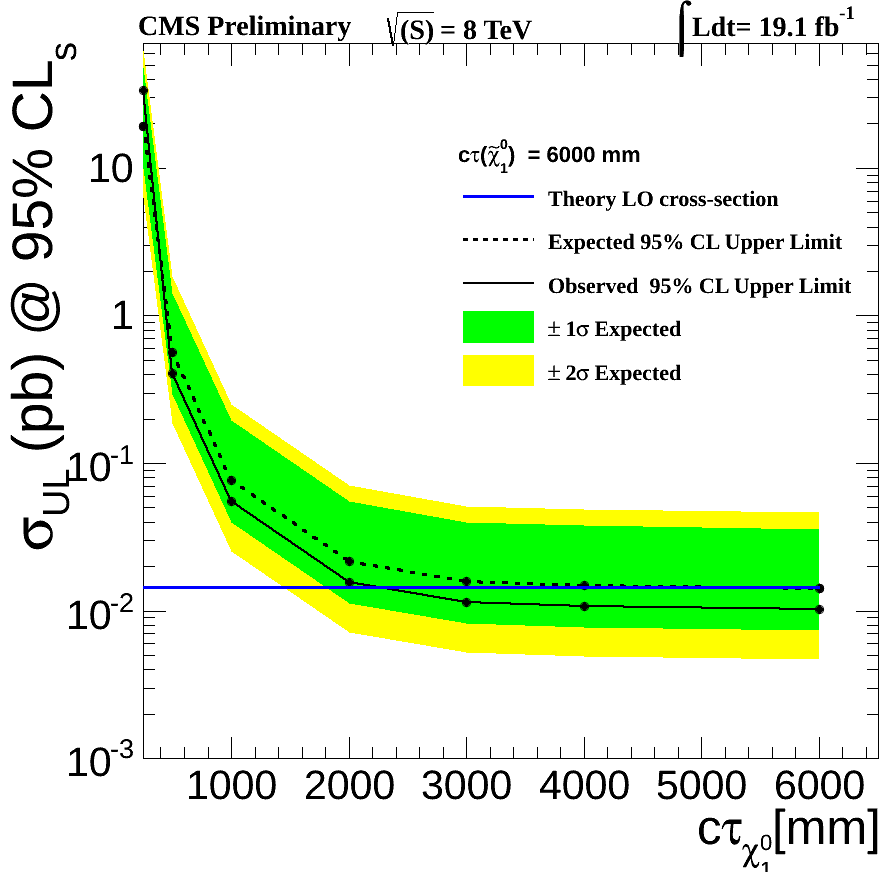
\includegraphics[width=5in]{THESISPLOTS/XsecTimesBR_Uplimit_Asymptotic_65Toys.png}}
\captionof{figure}{Neutralino production cross section against proper delay length upper limit interpretation in SPS8 model.}
\label{fig:SPS8_Ulimit}
\end{center}
%%%%%%%%%%%%%%%%%%%%%%%%%%%%%%%%%%%%%%%%%%%%%%%%%%%%%%%%%%%%%%%%%%%%%%%%%%%%%%%%
